% Thanks to http://tex.stackexchange.com/a/30782/5645 for this
% example!
\documentclass{article}
\usepackage{amsmath}
\usepackage{ amssymb}
\usepackage{mathptmx}
\usepackage{tikz}
\usepackage{pgfplots}
\usepgfplotslibrary{polar}
\usepgfplotslibrary{fillbetween}
\usepackage{tkz-fct}
\usetikzlibrary{angles, quotes}
\usetikzlibrary{arrows.meta, arrows}
\usetikzlibrary{shapes.geometric}
\usetikzlibrary{external}
\tikzexternalize[prefix={external/}]

\tikzset{
    export as png/.style={
        external/system call/.add={}{
            && convert -density #1 -transparent white "\image.pdf" "\image.png"
        },
    },
    export as png/.default={200},
    % Arrow tips
    >=stealth,
}

% pgfplots settings
\input{colors}
\input{pgfplots}

\DeclareSymbolFont{symbolsb}{OMS}{cmsy}{m}{n}
\SetSymbolFont{symbolsb}{bold}{OMS}{cmsy}{b}{n}
\DeclareSymbolFontAlphabet{\mathcal}{symbolsb}

\def\req{\protect\rotatebox{90}{$\scriptstyle=$}}

\newcommand{\addaxes}{\draw (0em,1em) -- (0em,-1em)
                            (-1em,0em) -- (1em,0em);}
\newcommand{\stepfunc}{\draw[line width=1.5pt] (0.65em,0.65em) -- (0,0.65em) 
                                    -- (0,-0.65em) -- (-0.65em,-0.65em);}

\begin{document}

\tikzset{export as png}

\tikzsetnextfilename{arco-circunferencia}

% Author: Alfredo Sánchez Alberca (asalber@ceu.es)
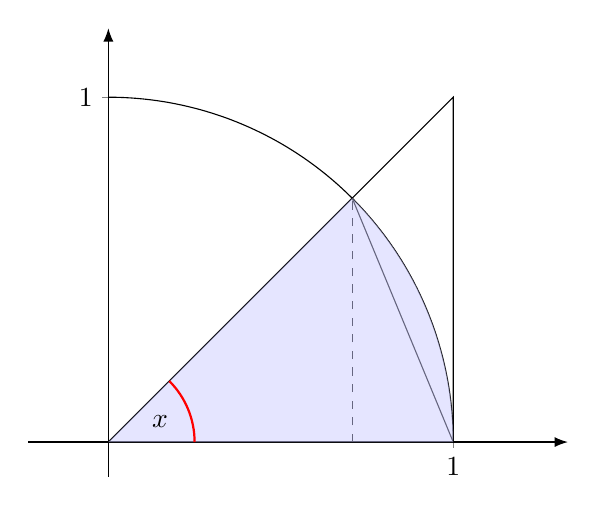
\begin{tikzpicture}
    \begin{axis}[
      axis equal,
      axis lines=center, % Place the axis at the center of the plot
      axis line style={-LaTeX}, % Add arrowheads to the axes
      xlabel={}, % Remove x-axis label
      ylabel={}, % Remove y-axis label
      xmin=-0.1, xmax=1.2,
      ymin=-0.1, ymax=1.2,
      xtick={0,1}, % Set x-axis tick positions
      ytick={0,1}, % Set y-axis tick positions
      ]
      \addplot [domain=0:pi/2, samples=100] ({cos(deg(x))}, {sin(deg(x))});
      \draw (0,0) -- ({cos(deg(pi/4))}, {sin(deg(pi/4))}) -- (1,0);
      \draw [dashed] ({cos(deg(pi/4))}, 0) -- ({cos(deg(pi/4))}, {sin(deg(pi/4))});
      \draw (0,0) -- (1, {tan(deg(pi/4))}) -- (1,0);
      \fill [blue!20, opacity=0.5] [dashed] (1,0) arc (0:45:1) -- (0,0);
      % Angle symbol and label
      \draw [red, thick] (0.25,0) arc (0:45:0.25);
      \node at (0.15,0.06) {$x$};
    \end{axis}
  \end{tikzpicture}

\end{document}